\let\negmedspace\undefined
\let\negthickspace\undefined
\documentclass[journal,12pt,onecolumn]{IEEEtran}
\usepackage{cite}
\usepackage{amsmath,amssymb,amsfonts,amsthm}
\usepackage{algorithmic}
\usepackage{graphicx}
\graphicspath{{./figs/}}
\usepackage{textcomp}
\usepackage{xcolor}
\usepackage{txfonts}
\usepackage{listings}
\usepackage{enumitem}
\usepackage{mathtools}
\usepackage{gensymb}
\usepackage{comment}
\usepackage{caption}
\usepackage[breaklinks=true]{hyperref}
\usepackage{tkz-euclide} 
\usepackage{listings}
\usepackage{gvv}                                        
%\def\inputGnumericTable{}                                 
\usepackage[latin1]{inputenc}     
\usepackage{xparse}
\usepackage{color}                                            
\usepackage{array}                                            
\usepackage{longtable}                                       
\usepackage{calc}                                             
\usepackage{multirow}
\usepackage{multicol}
\usepackage{hhline}                                           
\usepackage{ifthen}                                           
\usepackage{lscape}
\usepackage{tabularx}
\usepackage{array}
\usepackage{float}
\newtheorem{theorem}{Theorem}[section]
\newtheorem{problem}{Problem}
\newtheorem{proposition}{Proposition}[section]
\newtheorem{lemma}{Lemma}[section]
\newtheorem{corollary}[theorem]{Corollary}
\newtheorem{example}{Example}[section]
\newtheorem{definition}[problem]{Definition}
\newcommand{\BEQA}{\begin{eqnarray}}
\newcommand{\EEQA}{\end{eqnarray}}
\newcommand{\define}{\stackrel{\triangle}{=}}
\theoremstyle{remark}
\newtheorem{rem}{Remark}

\begin{document}

\title{
ASSIGNMENT 2: GATE 2012 \\
PI: PRODUCTION AND INDUSTRIAL ENGINEERING}
\author{AI25BTECH11034 -- Sujal Chauhan}
\date{}
\maketitle
\textbf{Q.1 -- Q. 25 carry one mark each.}

\begin{enumerate}
\vspace{1cm}
  % Q.1
  \item $\lim_{x \to 0} \left( \frac{1-\cos x}{x^2} \right)$ is \hfill{(GATE 2012)}
  \begin{enumerate}
    \item 1/4
    \item 1/2
    \item 1
    \item 2
  \end{enumerate}
\vspace{1cm}
  % Q.2
  \item For the spherical surface $x^2 + y^2 + z^2 = 1$, the unit outward normal vector at the point $\left(\tfrac{1}{\sqrt{2}}, \tfrac{1}{\sqrt{2}}, 0\right)$ is given by
  \hfill{(GATE 2012)}
  \begin{enumerate}
    \item $\tfrac{1}{\sqrt{2}} \, \hat{i} + \tfrac{1}{\sqrt{2}} \, \hat{j}$
    \item $\tfrac{1}{\sqrt{2}} \, \hat{i} - \tfrac{1}{\sqrt{2}} \, \hat{j}$
    \item $\hat{k}$
    \item $\tfrac{1}{\sqrt{3}} \, \hat{i} + \tfrac{1}{\sqrt{3}} \, \hat{j} + \tfrac{1}{\sqrt{3}} \, \hat{k}$
  \end{enumerate}
\vspace{1cm}
  % Q.3
  \item Consider the function $f(x) = |x|$ in the interval $-1 \leq x \leq 1$. At the point $x = 0$, $f(x)$ is
  \hfill{(GATE 2012)}
  \begin{enumerate}
    \item continuous and differentiable.
    \item non-continuous and differentiable.
    \item continuous and non-differentiable.
    \item neither continuous nor differentiable.
  \end{enumerate}
\vspace{1cm}
  % Q.4
  \item At $x=0$, the function $f(x) = x^2 + 1$ has
  \hfill{(GATE 2012)}
  \begin{enumerate}
    \item a maximum value
    \item a minimum value
    \item a singularity
    \item a point of inflection
  \end{enumerate}
\vspace{1cm}
  % Q.5
  \item The area enclosed between the straight line $y=x$ and the parabola $y=x^2$ in the $xy$-plane is
  \hfill{(GATE 2012)}
  \begin{enumerate}
    \item 1/6
    \item 1/4
    \item 1/3
    \item 1/2
  \end{enumerate}
\vspace{1cm}
  % Q.6
  \item For a long slender column of uniform cross section, the ratio of critical buckling load for the case with both ends clamped to the case with both ends hinged is
  \hfill{(GATE 2012)}
  \begin{enumerate}
    \item 1
    \item 2
    \item 4
    \item 8
  \end{enumerate}
\vspace{1cm}
  % Q.7
  \item A thin walled spherical shell is subjected to an internal pressure. If the radius of the shell is increased by 1\% and the thickness is reduced by 1\%, with the internal pressure remaining the same, the percentage change in the circumferential (hoop) stress is
  \hfill{(GATE 2012)}
  \begin{enumerate}
    \item 0
    \item 1
    \item 1.08
    \item 2.02
  \end{enumerate}
\vspace{1cm}
  % Q.8
  \item A cantilever beam of length L is subjected to a moment M at the free end. The moment of inertia of
the beam cross section on the neutral axis is $I$ and the young's modulus is$ E$. The magnitude of 
the maximum deflection is 
\hfill{(GATE 2012)}
  \begin{enumerate}
    \item $\dfrac{ML^2}{2EI}$
    \item $\dfrac{ML^2}{EI}$
    \item $\dfrac{2ML^2}{EI}$
    \item $\dfrac{4ML^2}{EI}$
  \end{enumerate}
\vspace{1cm}
  % Q.9
  \item A circular solid disc of uniform thickness $20 \,\text{mm}$, radius $200 \,\text{mm}$ and mass $20 \,\text{kg}$ is used as a flywheel. If it rotates at $600$ rpm, the kinetic energy of the flywheel, in Joules is
  \hfill{(GATE 2012)}
  \begin{enumerate}
    \item 395
    \item 790
    \item 1580
    \item 3160
  \end{enumerate}
\vspace{1cm}

% Q.10
\item  In the mechanism given below, if the angular velocity of the eccentric circular disc is 1 rad/s, the angular velocity (rad/s) of the follower link for the instant shown in the figure is
\hfill{(GATE 2012)}

\textit{Note: All dimensions are in mm.}

\begin{figure}[h!]
\centering
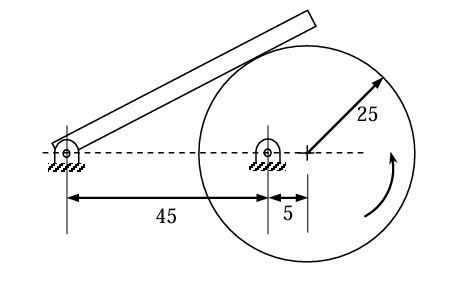
\includegraphics[width=0.5\textwidth]{GATE-PI-2012/10-GATE-PI-2012.png}
\caption{}
\label{q10}
\end{figure}

\begin{enumerate}
\item 0.05
\item 0.1
\item 5.0
\item 10.0
\end{enumerate}
\vspace{1cm}
% Q.11
\item Steam enters an adiabatic turbine operating at steady state with an enthalpy of 3251.0 kJ/kg and leaves as a saturated mixture at 15 kPa with quality (dryness fraction) 0.9. The enthalpies of the saturated liquid and vapor at 15 kPa are $h_f = 225.94 \, kJ/kg$ and $h_g = 2598.3 \, kJ/kg$ respectively. The mass flow rate of steam is 10 kg/s. Kinetic and potential energy changes are negligible. The power output of the turbine in MW is
\hfill{(GATE 2012)}

\begin{enumerate}
\item 6.5
\item 8.9
\item 9.1
\item 27.0
\end{enumerate}
\vspace{1cm}
% Q.12
\item  An ideal gas of mass $m$ and temperature $T_1$ undergoes a reversible isothermal process from an initial pressure $P_1$ to final pressure $P_2$. The heat loss during the process is $Q$. The entropy change $\Delta S$ of the gas is
\hfill{(GATE 2012)}

\begin{enumerate}
\item $mR \ln \left(\frac{P_2}{P_1}\right)$
\item $mR \ln \left(\frac{P_1}{P_2}\right)$
\item $mR \ln \left(\frac{P_2}{P_1}\right) - \frac{Q}{T_1}$
\item zero
\end{enumerate}
\vspace{1cm}
% Q.13
\item For an opaque surface, the absorptivity $(\alpha)$, transmissivity $(\tau)$ and reflectivity $(\rho)$ are related by the equation:
\hfill{(GATE 2012)}

\begin{enumerate}
\item $\alpha + \rho = \tau$
\item $\rho + \alpha + \tau = 0$
\item $\alpha + \rho = 1$
\item $\alpha + \rho = 0$
\end{enumerate}
\vspace{1cm}
% Q.14
\item  Which of the following configurations has the highest fin effectiveness?
\hfill{(GATE 2012)}

\begin{enumerate}
\item Thin, closely spaced fins
\item Thin, widely spaced fins
\item Thick, widely spaced fins
\item Thick, closely spaced fins
\end{enumerate}
\vspace{1cm}
% Q.15
\item  Oil flows through a 200 mm diameter horizontal cast iron pipe (friction factor, $f=0.0225$) of length 500 m. The volumetric flow rate is $0.2 \, m^3/s$. The head loss (in m) due to friction is (assume $g=9.81 \, m/s^2$)
\hfill{(GATE 2012)}

\begin{enumerate}
\item 116.5
\item 0.116
\item 12.2
\item 232.36
\end{enumerate}
\vspace{1cm}
% Q.16
\item  A solid cylinder of diameter 100 mm and height 50 mm is forged between two frictionless flat dies until the height is 25 mm. The percentage change in diameter is
\hfill{(GATE 2012)}

\begin{enumerate}
\item 18.6
\item 20.0
\item 41.4
\item 52.6
\end{enumerate}

\vspace{1cm}
% Q.17
\item Q.17 In an interchangeable assembly, shafts of size $25.000^{-0.010}_{+0.030}$ mm mate with holes of size $25.000^{+0.020}_{+0.020}$ mm. The maximum interference (in microns) in the assembly is
\hfill{(GATE 2012)}

\begin{enumerate}
\item 40
\item 30
\item 20
\item 10
\end{enumerate}

\vspace{1cm}
% Q.18
\item A CNC vertical milling machine has to cut a straight slot of 10 mm width and 2 mm depth by a cutter of 10 mm diameter between points (0, 0) and (100, 100) on the $XY$ plane (dimensions in mm). The feed rate used for milling is 50 mm/min. Milling time for the slot (in seconds) is\\
\hfill{(GATE 2012)}

\begin{enumerate}
\item 120
\item 170
\item 180
\item 240
\end{enumerate}

\vspace{1cm}
% Q.19
\item Match the following metal forming processes with their associated stresses in the workpiece.
\hfill{(GATE 2012)}

\begin{center}
\begin{tabular}{ll}
Metal forming process & Type of stress \\
1. Coining       & P. Tensile \\
2. Wire Drawing  & Q. Shear \\
3. Blanking      & R. Tensile and compressive \\
4. Deep Drawing  & S. Compressive \\
\end{tabular}
\end{center}

\begin{enumerate}
\item 1-S, 2-P, 3-Q, 4-R
\item 1-S, 2-P, 3-R, 4-Q
\item 1-P, 2-Q, 3-S, 4-R
\item 1-P, 2-R, 3-Q, 4-S
\end{enumerate}

\vspace{1cm}
% Q.20
\item During \textit{normalizing} process of steel, the specimen is heated
\hfill{(GATE 2012)}

\begin{enumerate}
\item between the upper and lower critical temperature and cooled in still air.
\item above the upper critical temperature and cooled in furnace.
\item above the upper critical temperature and cooled in still air.
\item between the upper and lower critical temperature and cooled in furnace.
\end{enumerate}

\vspace{1cm}
% Q.21
\item  In abrasive jet machining, as the distance between the nozzle tip and the work surface increases, the material removal rate
\hfill{(GATE 2012)}

\begin{enumerate}
\item increases continuously.
\item decreases continuously.
\item decreases, becomes stable and then increases.
\item increases, becomes stable and then decreases.
\end{enumerate}

\vspace{1cm}
% Q.22
\item  Which one of the following is NOT a decision taken during the aggregate production planning stage?
\hfill{(GATE 2012)}

\begin{enumerate}
\item Scheduling of machines
\item Amount of labour to be committed
\item Rate at which production should happen
\item Inventory to be carried forward
\end{enumerate}

\vspace{1cm}
% Q.23
\item  Which one of the following is NOT associated with the process of new product development?
\hfill{(GATE 2012)}

\begin{enumerate}
\item QFD
\item FEMA
\item KANBAN
\item DFMA
\end{enumerate}
\vspace{1cm}
% Q.24
\item  A process needs to be standardized for method and time. Which one of the following represents the sequence of work study experiments?
\hfill{(GATE 2012)}

\begin{enumerate}
\item Time study followed by method study
\item Only time study
\item Time study and method study simultaneously
\item Method study followed by time study
\end{enumerate}

\vspace{1cm}
% Q.25
\item  Reduction in the variability of manufactured product characteristics will definitely result in observations close to
\hfill{(GATE 2012)}

\begin{enumerate}
\item the upper control limit in $\overline{X}$ chart.
\item the lower control limit in $\overline{X}$ chart.
\item the lower control limit in $R$ chart.
\item the center line in $R$ chart.
\end{enumerate}
\newpage
\vspace{1cm}
% Q.26
\item  The system of algebraic equations given below has
\[
x + 2y + z = 4 \\
2x + y + 2z = 5 \\
x - y + z = 1
\]
\hfill{(GATE 2012)}

\begin{enumerate}
\item A unique solution of $x=1, y=1$ and $z=1$.
\item Only two solutions of $(x=1, y=1, z=1)$ and $(x=2, y=1, z=0)$.
\item Infinite number of solutions.
\item No feasible solution.
\end{enumerate}

\vspace{1cm}
% Q.27
\item  For the matrix $A=\myvec{5 & 3 \\ 1 & 3}$, ONE of the normalized eigen vectors is given as
\hfill{(GATE 2012)}

\begin{enumerate}
\item $\myvec{\tfrac{1}{2} \\ \tfrac{\sqrt{3}}{2}}$
\item $\myvec{\tfrac{1}{\sqrt{2}} \\ -\tfrac{1}{\sqrt{2}}}$
\item $\myvec{\tfrac{3}{\sqrt{10}} \\ -\tfrac{1}{\sqrt{10}}}$
\item $\myvec{\tfrac{1}{\sqrt{5}} \\ \tfrac{2}{\sqrt{5}}}$
\end{enumerate}

\vspace{1cm}
% Q.28
\item  Consider the differential equation 
\[
x^2 \frac{d^2 y}{dx^2} + x \frac{dy}{dx} - 4y = 0
\]
with the boundary conditions of $y(0)=0$ and $y(1)=1$. The complete solution of the differential equation is
\hfill{(GATE 2012)}

\begin{enumerate}
\item $x^2$
\item $\sin\left(\tfrac{\pi x}{2}\right)$
\item $e^x \sin\left(\tfrac{\pi x}{2}\right)$
\item $e^x \sin\left(\tfrac{\pi x}{2}\right)$
\end{enumerate}

\vspace{1cm}
% Q.29
\item  The inverse Laplace transform of the function $F(s)=\tfrac{1}{s(s+1)}$ is given by
\hfill{(GATE 2012)}

\begin{enumerate}
\item $f(t) = \sin t$
\item $f(t) = e^{-t} \sin t$
\item $f(t) = e^t$
\item $f(t) = 1 - e^{-t}$
\end{enumerate}

\vspace{1cm}
% Q.30
\item  A box contains 4 red balls and 6 black balls. Three balls are selected randomly from the box one after another, without replacement. The probability that the selected set contains one red ball and two black balls is
\hfill{(GATE 2012)}

\begin{enumerate}
\item 1/20
\item 1/12
\item 3/10
\item 1/2
\end{enumerate}

\vspace{1cm}
% Q.31
\item  The state of stress at a point under plane stress condition is
\[
\sigma_{xx} = 40 \, \text{MPa}, \quad \sigma_{yy} = 100 \, \text{MPa}, \quad \tau_{xy} = 40 \, \text{MPa}.
\]
The radius of the Mohra's circle representing the given state of stress in MPa is
\hfill{(GATE 2012)}

\begin{enumerate}
\item 40
\item 50
\item 60
\item 100
\end{enumerate}
\vspace{1cm}
% Q.32
\item A force of 400 $N$ is applied to the brake drum of 0.5 m diameter in a band-brake system as shown in the figure, where the wrapping angle is $180^\circ$. If the coefficient of friction between the drum and the band is 0.25, the braking torque applied, in $N.m$ is
\hfill{(GATE 2012)}

\begin{figure}[h!]
\centering
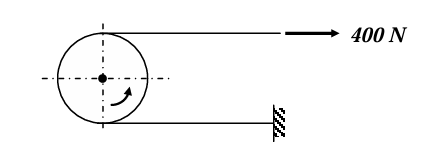
\includegraphics[width=0.4\textwidth]{GATE-PI-2012/32-GATE-PI-2012.png}
\caption{}
\label{q32}
\end{figure}

\begin{enumerate}
\item 100.6
\item 54.4
\item 22.1
\item 15.7
\end{enumerate}
\vspace{1cm}

% Q.33
\item Water ($C_p=4.18 \, kJ/kgK$) at $80^\circ C$ enters a counterflow heat exchanger with a mass flow rate of $0.5 \, kg/s$. Air ($C_p = 1 \, kJ/kgK$) enters at $30^\circ C$ with a mass flow rate of $2.09 \, kg/s$. If the effectiveness of the heat exchanger is $0.8$, the LMTD (in $^\circ C$) is
\hfill{(GATE 2012)}

\begin{enumerate}
\item 40
\item 20
\item 10
\item 5
\end{enumerate}
\vspace{1cm}

% Q.34
\item Consider two infinitely long \textit{thin} concentric tubes of circular cross section as shown in the figure. If $D_1$ and $D_2$ are the diameters of the inner and outer tubes respectively, then the view factor $F_{22}$ is
\hfill{(GATE 2012)}

\begin{figure}[h!]
\centering
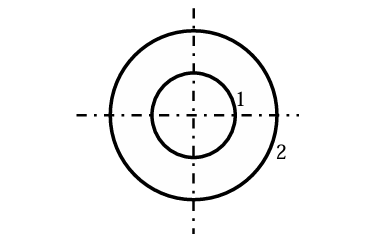
\includegraphics[width=0.35\textwidth]{GATE-PI-2012/34-GATE-PI-2012.png}
\caption{}
\label{q34}
\end{figure}

\begin{enumerate}
\item $\left(\tfrac{D_2}{D_1}\right) - 1$
\item zero
\item $\tfrac{D_1}{D_2}$
\item $1 - \left(\tfrac{D_1}{D_2}\right)$
\end{enumerate}
\vspace{1cm}

% Q.35
\item A large tank with a nozzle attached contains three immiscible, inviscid fluids as shown. Assuming that the changes in $h_1, h_2,$ and $h_3$ are negligible, the instantaneous discharge velocity is
\hfill{(GATE 2012)}

\begin{figure}[h!]
\centering
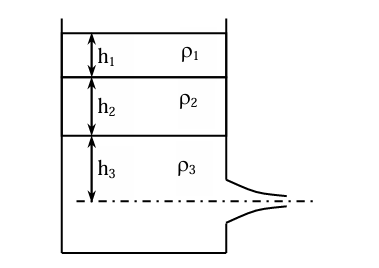
\includegraphics[width=0.35\textwidth]{GATE-PI-2012/35-GATE-PI-2012.png}
\caption{}
\label{q35}
\end{figure}

\begin{enumerate}
\item $\sqrt{2 g h_1 \left(1 + \tfrac{\rho_1}{\rho_3}\tfrac{h_1}{h_3} + \tfrac{\rho_2}{\rho_3}\tfrac{h_2}{h_3}\right)}$
\item $\sqrt{2 g (h_1 + h_2 + h_3)}$
\item $\sqrt{2 g \left(\tfrac{\rho_1 h_1 + \rho_2 h_2 + \rho_3 h_3}{\rho_1 + \rho_2 + \rho_3}\right)}$
\item $\sqrt{2 g \left(\tfrac{\rho_1 h_1 h_2 + \rho_2 h_2 h_3 + \rho_3 h_3 h_1}{\rho_1 h_1 + \rho_2 h_2 + \rho_3 h_3}\right)}$
\end{enumerate}
\vspace{1cm}
% Q.36
\item In a DC arc welding operation, the voltage-arc length characteristic was obtained as $V_{arc} = 20 + 5l$ where the arc length $l$ was varied between $5 \, mm$ and $7 \, mm$. Here $V_{arc}$ denotes the arc voltage in $Volts$. The arc current was varied from $400 \, A$ to $500 \, A$. Assuming linear power source characteristic, the \textit{open circuit voltage} and the \textit{short circuit current} for the welding operation are
\hfill{(GATE 2012)}

\begin{enumerate}
\item 45 V, 450 A
\item 75 V, 750 A
\item 95 V, 950 A
\item 150 V, 1500 A
\end{enumerate}
\vspace{1cm}

% Q.37
\item In a single pass rolling process using $410 \, mm$ diameter steel rollers, a strip of width $140 \, mm$ and thickness $8 \, mm$ undergoes $10\%$ reduction of thickness. The \textit{angle of bite} in radians is
\hfill{(GATE 2012)}

\begin{enumerate}
\item 0.006
\item 0.031
\item 0.062
\item 0.600
\end{enumerate}
\vspace{1cm}

% Q.38
\item A mould having dimensions $100 \, mm \times 90 \, mm \times 20 \, mm$ is filled with molten metal through a gate as shown in the figure. For height $h$ and cross-sectional area $A$, the mould filling time is $t_1$. The height is now quadrupled and the cross-sectional area is halved. The corresponding filling time is $t_2$. The ratio $t_2/t_1$ is
\hfill{(GATE 2012)}

\begin{figure}[h!]
\centering
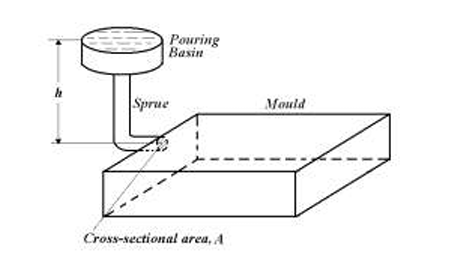
\includegraphics[width=0.4\textwidth]{GATE-PI-2012/38-GATE-PI-2012.png}
\caption{}
\label{q38}
\end{figure}

\begin{enumerate}
\item $\tfrac{1}{\sqrt{2}}$
\item 1
\item $\sqrt{2}$
\item 2
\end{enumerate}
\vspace{1cm}

% Q.39
\item A thin square plate $ABCD$ with side of unit length is kept in the $X$-$Y$ plane as shown in the figure. The plate is first rotated by $30^\circ$ in the anti-clockwise direction about the $Z$-axis with $A$ fixed at the origin. The plate is then rotated by $90^\circ$ in the anti-clockwise direction about the $X$-axis with $A$ fixed at the origin. The final co-ordinates of $C$ are
\hfill{(GATE 2012)}

\begin{figure}[h!]
\centering
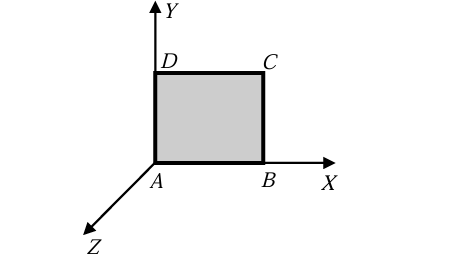
\includegraphics[width=0.35\textwidth]{GATE-PI-2012/39-GATE-PI-2012.png}
\caption{}
\label{q39}
\end{figure}

\begin{enumerate}
\item (1.366, 0.366, 0.0)
\item (0.0, 1.366, 0.366)
\item (1.366, 0.0, 0.366)
\item (0.366, 0.0, 1.366)
\end{enumerate}
\vspace{1cm}

% Q.40
\item A sine bar has a length of $250 \, mm$. Each roller has a diameter of $20 \, mm$. During taper angle measurement of a component, the height from the surface plate to the centre of a roller is $100 \, mm$. The calculated taper angle (in degrees) is
\hfill{(GATE 2012)}

\begin{enumerate}
\item 21.1
\item 22.8
\item 23.6
\item 68.9
\end{enumerate}
\vspace{1cm}

% Q.41
\item Match the following plastic products with their most appropriate materials. 
\hfill{(GATE 2012)}

\begin{tabular}{ll}
Products & Materials \\
1. Gears & P. Polymethylmethacrylate (PMMA) \\
2. Helmets & Q. Polyamides (PA) \\
3. Lenses & R. Polyethylene (PE) \\
4. Food packaging & S. Acrylonitrile-butadiene-styrene (ABS) \\
\end{tabular}

\begin{enumerate}
\item  1-Q, 2-R, 3-S, 4-P
\item  1-S, 2-P, 3-Q, 4-R
\item  1-P, 2-Q, 3-R, 4-S
\item  1-Q, 2-S, 3-P, 4-R
\end{enumerate}
\vspace{1cm}

% Q.42
\item In a shaping process, the number of double strokes per minute is 30 and the quick return ratio is 0.6. 
If the length of the stroke is $250 \, mm$, the average cutting velocity in $m/min$ is  
\hfill{(GATE 2012)}

\begin{enumerate}
\item 3.0
\item 4.5
\item 7.5
\item 12.0
\end{enumerate}
\vspace{1cm}

% Q.43
\item For a linear programming problem, the set of constraints $x+y \leq 2, \; 3x+5y \geq 15, \; x \geq 0 \;\; \text{and} \;\; y \geq 0$ leads to  
\hfill{(GATE 2012)}

\begin{enumerate}
\item an infeasible solution.
\item a unique optimal solution.
\item multiple but finite optimal solutions.
\item infinite optimal solutions.
\end{enumerate}
\vspace{1cm}

% Q.44
\item A milk vendor incurs an overstocking cost of Rs. $2$ per litre and a shortage cost of Rs. $0.5$ per litre. 
The demand is uniformly distributed between $1 \, litre$ and $6 \, litres$. Using the Newsvendor Model, the maximum quantity of milk in litre(s) the vendor should order is  
\hfill{(GATE 2012)}

\begin{enumerate}
\item 2
\item 6
\item 1
\item 3
\end{enumerate}
\vspace{1cm}

% Q.45
\item The specification limits for the weight of a product are $13.1 \, kg$ and $15 \, kg$. 
If the process has a variance of weight $0.05 \, kg^2$, then the process capability index is  
\hfill{(GATE 2012)}

\begin{enumerate}
\item 6.3
\item 1.9
\item 1.4
\item 8.6
\end{enumerate}
\vspace{1cm}

% Q.46
\item On an average, there are $30$ customers in a queue. 
If the arrival rate of customers into the system is $16$ customers per hour and on average $32$ customers leave the system per hour, then the average number of customers in the system is  
\hfill{(GATE 2012)}

\begin{enumerate}
\item 16.5
\item 30.5
\item 32.0
\item 46.0
\end{enumerate}
\vspace{1cm}

% Q.47
\item Data for four jobs that need to be processed on a single machine are given below. 
\hfill{(GATE 2012)}

\begin{tabular}{|c|c|c|}
\hline
Job & Processing time (days) & Due date (days) \\
\hline
P & 12 & 20 \\
Q & 9 & 40 \\
R & 21 & 30 \\
S & 10 & 19 \\
\hline
\end{tabular}


All the four jobs are available at time zero. If the jobs are scheduled using the Earliest Due Date (EDD) algorithm, then the job with maximum tardiness is  

\begin{enumerate}
\item P
\item Q
\item R
\item S
\end{enumerate}
\vspace{1cm}
\textbf{Common Data Questions }\\
\textbf{Common Data for Questions 48 and 49:   }\\
Two steel truss members, AC and BC, each having cross sectional area of $100 \, mm^2$, 
are subjected to a horizontal force $F$ as shown in figure. All the joints are hinged.  

\begin{figure}[h]
\centering
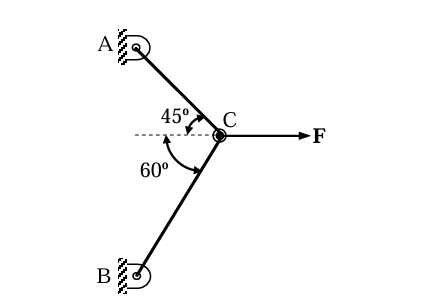
\includegraphics[width=0.4\textwidth]{GATE-PI-2012/48-GATE-PI-2012.png} 
\caption{}
\label{}
\end{figure}

% Q.48
\item The maximum force $F$ in $kN$ that can be applied at C such that the axial stress in any of the truss members 
DOES NOT exceed $100 \, MPa$ is  
\hfill{(GATE 2012)}

\begin{enumerate}
\item 8.17
\item 11.15
\item 14.14
\item 22.30
\end{enumerate}
\vspace{1cm}

% Q.49
\item IF $F = 1 \, kN$, the magnitude of the vertical reaction force developed at the point B in $kN$ is  
\hfill{(GATE 2012)}

\begin{enumerate}
\item 0.63
\item 0.32
\item 1.26
\item 1.46
\end{enumerate}
\vspace{1cm}

%  Q.50 and Q.51
\textbf{Common Data for Questions 50 and 51:   }\\
Data for a plain milling operation are given below.  

\begin{tabular}{ll}
Length of workpiece & $200 \, mm$ \\
Cutter diameter & $100 \, mm$ \\
No. of teeth & $4$ \\
Cutter speed & $100 \, rpm$ \\
Feed & $200 \, mm/min$ \\
Depth of cut & $2 \, mm$ \\
Total clearance (entry and exit) & $5 \, mm$ \\
\end{tabular}

% Q.50
\item Mean undeformed chip thickness (in microns) is  
\hfill{(GATE 2012)}

\begin{enumerate}
\item 142
\item 100
\item 71
\item 50
\end{enumerate}
\vspace{1cm}

% Q.51
\item Machining time for a single pass (in seconds) is  
\hfill{(GATE 2012)}

\begin{enumerate}
\item 60
\item 66
\item 126
\item 150
\end{enumerate}
\vspace{1cm}


% Q.52 and Q.53
\textbf{Linked Answer Questions }\\
\textbf{Statement for Linked Answer Questions 52 and 53:    }\\
\textbf In an EDM process using RC relaxation circuit, a $12 \, mm$ diameter through hole is made in a steel plate of $50 \, mm$ thickness using a graphite tool and kerosene as dielectric. Assume discharge time to be negligible. Machining is carried out under the following conditions:
\begin{itemize}
  \item Resistance: $40 \, \Omega$
  \item Capacitance: $20 \, \mu F$
  \item Supply voltage: $220 \, V$
  \item Discharge voltage: $110 \, V$
\end{itemize}

% Q.52
\item The time for one cycle, in milliseconds, is  
\hfill{(GATE 2012)}

\begin{enumerate}
\item 0.55
\item 0.32
\item 0.89
\item 0.24
\end{enumerate}
\vspace{1cm}

% Q.53
\item Average power input (in kW) is  
\hfill{(GATE 2012)}

\begin{enumerate}
\item 0.373
\item 0.137
\item 0.218
\item 0.500
\end{enumerate}
\vspace{1cm}

%  Q.54 and Q.55
\textbf{Statement for Linked Answer Questions 54 and 55: }\\
\textbf In a particular year, an organization earns cash revenues of Rs. $2{,}00{,}000$. Total material and labour expenses are Rs. $1{,}09{,}000$. The depreciation claimed on the equipment is Rs. $25{,}000$. The tax rate is $20\%$.

% Q.54
\item The profit after tax (PAT) is  
\hfill{(GATE 2012)}

\begin{enumerate}
\item Rs. 92,800
\item Rs. 66,200
\item Rs. 72,800
\item Rs. 52,800
\end{enumerate}
\vspace{1cm}

% Q.55
\item The net cash flow is  
\hfill{(GATE 2012)}

\begin{enumerate}
\item Rs. 97,800
\item Rs. 77,800
\item Rs. 66,000
\item Rs. 72,800
\end{enumerate}
\vspace{1cm}







\end{enumerate}

\end{document}